\documentclass[a4paper, 12pt, notitlepage]{article}
\usepackage[utf8]{inputenc}
\usepackage[T1]{fontenc}
\usepackage[english]{babel}
\usepackage{amsmath, amsfonts, amssymb, amsthm, mathtools}
\usepackage{pythonhighlight}
\usepackage{listings}
\usepackage{float}
\usepackage{makeidx}
\usepackage{siunitx}
\usepackage{array}
\usepackage[top=1in]{geometry}  
\usepackage{caption}
\usepackage{subcaption}
\usepackage{graphicx}
\graphicspath{{C:/Users/skief/Documents/UiT/semester8/HEIMDALL/figures}}
\usepackage{wrapfig}
\usepackage{hyperref}
\usepackage[backend=biber, sorting = nty]{biblatex}
\usepackage{biblatex}

\addbibresource{ref.bib}

\begin{document}
\author{Selma Kiefersauer}
\title{FYS-3003 and FYS-3002: Heimdall Campaign}
\maketitle

\section{UHF and VHF}

\begin{figure}[H]
	\centering
	\caption{UHF (beata) and VHF (bella) plots from the experiment}
	\begin{subfigure}[b]{0.45\textwidth}
		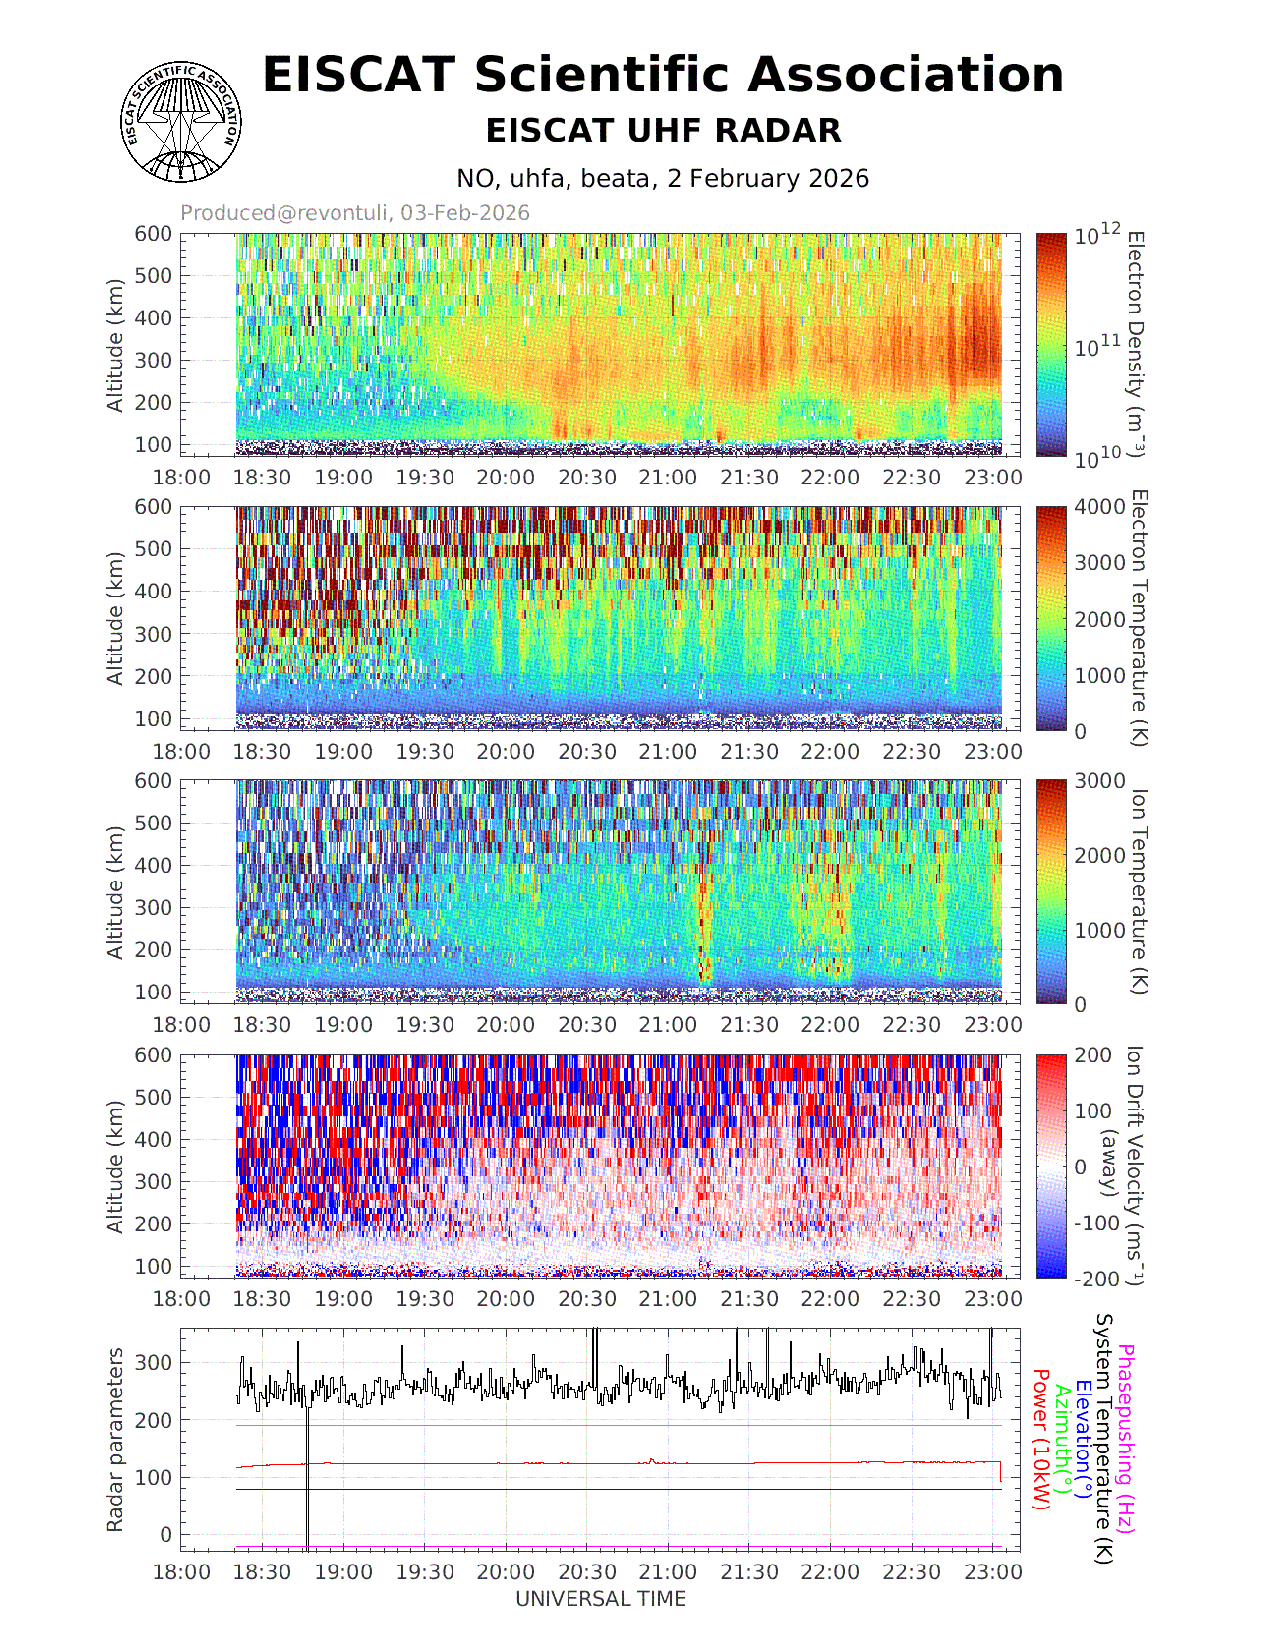
\includegraphics[width=\textwidth]{2026-02-02_beata_30_18-23@uhfa.png}
	\end{subfigure}
	\begin{subfigure}[b]{0.45\textwidth}
		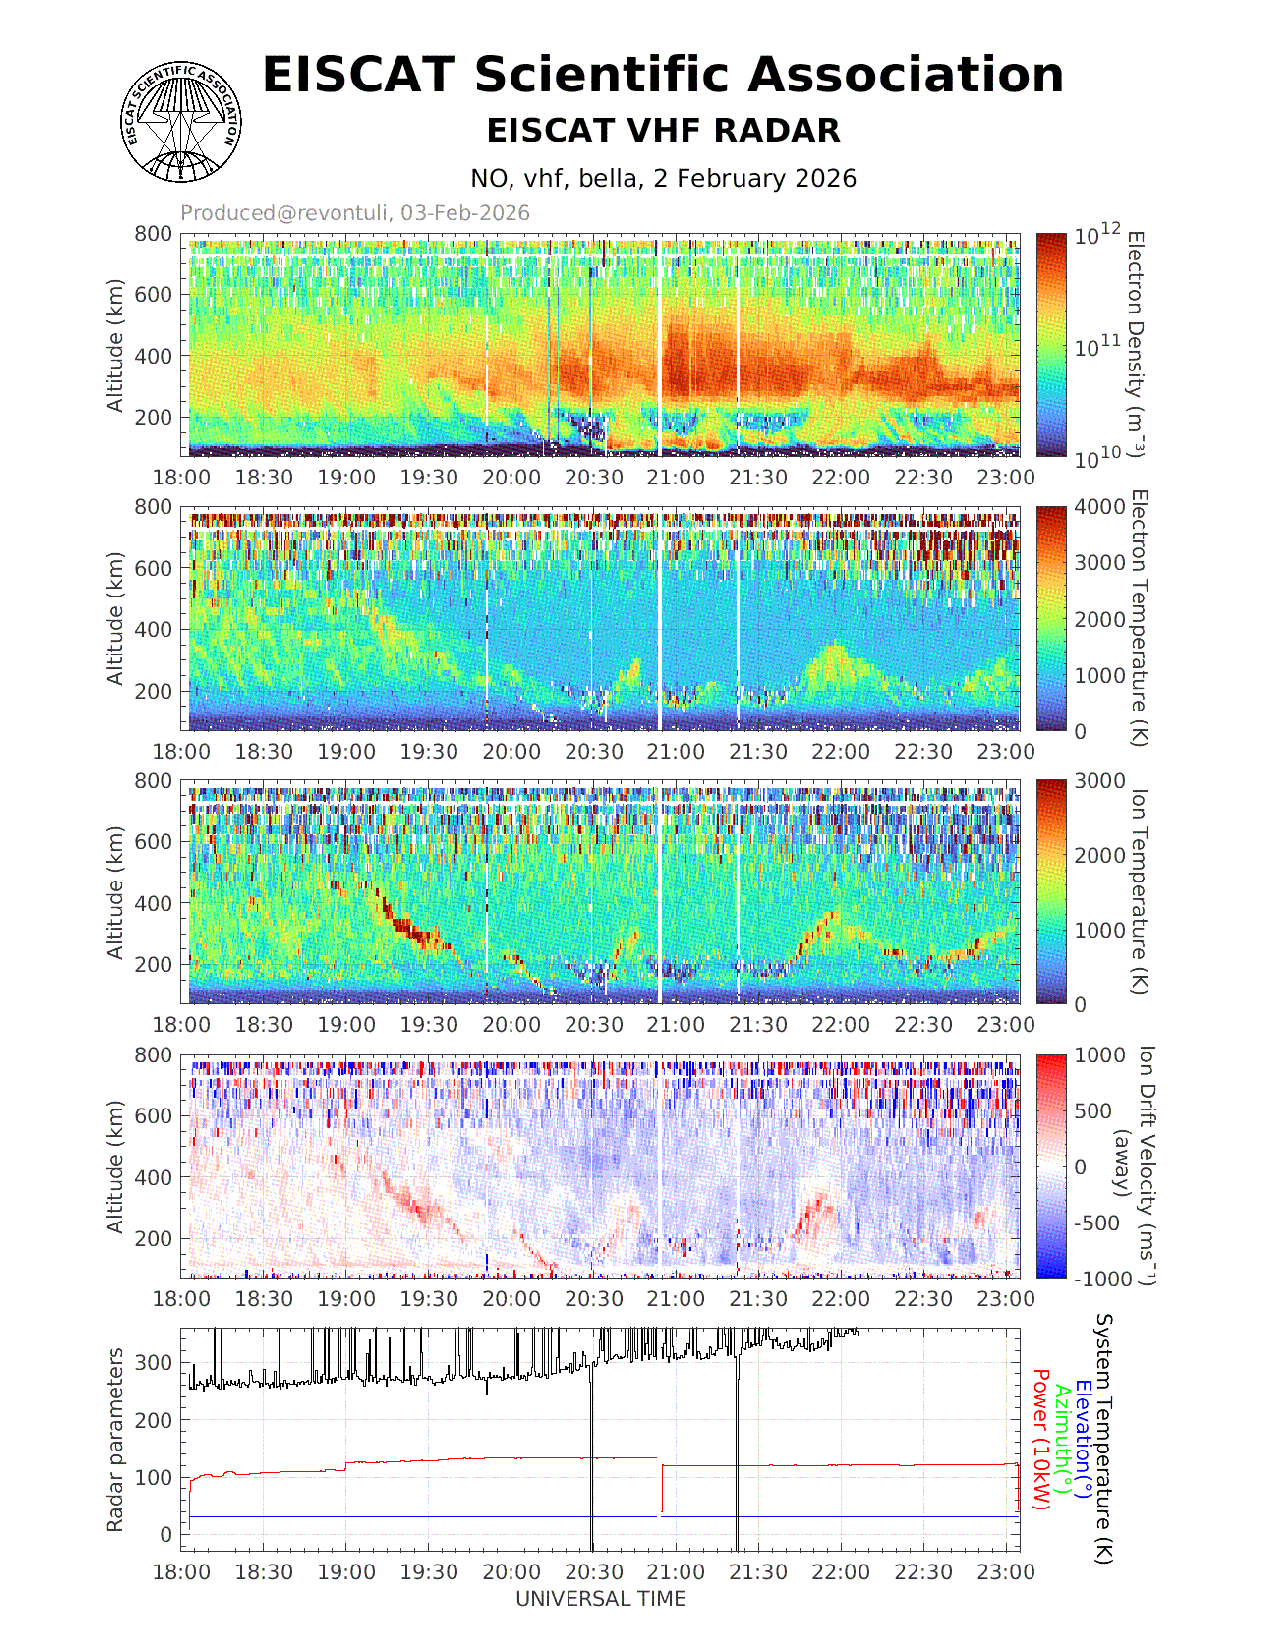
\includegraphics[width=\textwidth]{2026-02-02_bella_30_18-23@vhf.png}
	\end{subfigure}
\end{figure}

The UHF antenna is a 32m parabolic dish antenna that measures along the magnetic field lines (almost straight up). It operates at about 929 MHz. The program run is "beata" (range 51 - 696km, resolution 5.0s). 

The VHF antenna is a rectangular four times 30x40m dish that measures due north at an upward angle of 30degrees from the horizon. It operates at about 224 MHz. The program used in the experiment is "bella" (range 69 - 1352km, resolution 3.6s). 

Can I plot the VHF data on a map? Where and when are the electron enhancements exaclty?

\clearpage
\section{Solar Wind Data}

From ACE: 

\begin{figure}[H]
	\centering
	
\includegraphics[width=\textwidth]{ACE_data}
\end{figure}

What is the time delay from ACE to earth? ACE is located at a distance of 1.5 million km from earth. The solar wind mean velocity in the plotted time interval is 303 km/s and this means it takes about 4950s or 82.5 min. 

Based on this estimate I added the points  which IMF measurement corresponds to the pictured TEC and SuperDARN data in section 3. The IMF corresponding to 19:00 UT has strong -By, no Bz and medium +Bx, at 21:00UT we have strong -By, no Bz and medium +By, at 22:00UT the IMF has strong -By, some -Bx and +Bz. At 23:00 we still have strong -By and virtually no Bz and Bx components.  Expected convection patterns: (\cite{WeimerB} \cite{ClusterEDI2})
\begin{figure}[H]
	\centering
	
\includegraphics[width=\textwidth]{ConvecIMF}
\end{figure}


\clearpage
\section{TEC from GNSS and SuperDARN}

TEC: It would be interesting to look at the TEC data during the experiment, especially north of Troms{\o}. Is there any indication where the electron enhancements come from? Is there some interesting convection pattern indicated?
\begin{figure}[H]
	\centering
	\caption{TEC from GNSS polar view.}
	\begin{subfigure}[b]{0.56\textwidth}
		
\includegraphics[width=\textwidth]{TEC1910.png}
	\end{subfigure}
	\begin{subfigure}[b]{0.43\textwidth}
		
\includegraphics[width=\textwidth]{TEC2100.png}
	\end{subfigure}
	\begin{subfigure}[b]{0.56\textwidth}
		
\includegraphics[width=\textwidth]{TEC2200.png}
	\end{subfigure}
	\begin{subfigure}[b]{0.43\textwidth}
		
\includegraphics[width=\textwidth]{TEC2300.png}
	\end{subfigure}
\end{figure}

Super Darn plots from the same time intervall
\begin{figure}[H]
	\centering
	\caption{SuperDarn Plots from the VT SuperDarn Convection Maps plotting tool.}
	\begin{subfigure}[b]{0.47\textwidth}
		
\includegraphics[width=\textwidth]{SDarn1900.png}
	\end{subfigure}
	\begin{subfigure}[b]{0.45\textwidth}
		
\includegraphics[width=\textwidth]{SDarn2100.png}
	\end{subfigure}
	\begin{subfigure}[b]{0.47\textwidth}
		
\includegraphics[width=\textwidth]{SDarn2200.png}
	\end{subfigure}
	\begin{subfigure}[b]{0.45\textwidth}
		
\includegraphics[width=\textwidth]{SDarn2300.png}
	\end{subfigure}
\end{figure}

\begin{figure}[H]
	\centering
	
\includegraphics[width=0.8\textwidth]{electron_densities_EISCAT.png}
\end{figure}

\begin{figure}[H]
	\centering
	
\includegraphics[width=0.8\textwidth]{2dcorr}
\end{figure}

\begin{figure}[H]
	\centering
	
\includegraphics[width=0.8\textwidth]{1dcorr}
\end{figure}
\clearpage

\section{Swarm satellites}
Swarm A and B:  Swarm B passes the radar beam (VHF) around 21.36 UTC.
\begin{figure}[H]
	\centering
	
\includegraphics[width=0.75\textwidth]{SwarmTrajec.png}
\end{figure}
 What would be interesting to compare?\\
Use Swarm to look at convection patterns by looking at plasma drift velocity (Langmuir probes and Thermal Ion imagers).


\section{Other instruments}

\begin{figure}[H]
	\centering
	
\includegraphics[width=0.8\textwidth]{Stackplot_Magnetometers020226.pdf}
\end{figure}

All-sky cameras Ramfjordmoen show some Aurora but very faint. All cameras around didn't show anything as it was cloudy in Skibotn, Longyearbyen, Ny-\aa lesund.

\url{https://tromsoe-ai.cei.uec.ac.jp/#/}


\section{Questions}

Why did the electron density peak around midnight?\\
Can it be related to convection patterns?\\
\cite{WeimerA}, \cite{WeimerB}, \cite{ClusterEDI}, \cite{ClusterEDI2}, \cite{Cowley1992}, \cite{sporadicF}, \cite{SwarmSuperDARN}, \cite{enhancedF}

\printbibliography[title={List of Papers}]
\end{document}